\documentclass{article}
\usepackage{graphicx}

\begin{document}
\begin{quote}
``The true engineering experience occurs not with your eyes and ears, 
but rather with your fingers and elbows. In other words, engineering 
education does not happen by listening in class or reading a book; 
rather it happens by designing under the watchful eyes of a patient 
mentor. So, go build something, then show it to someone you res\-pect!''\\
V\'ease Preface to Volume del libro \cite{Valvano}.
\end{quote}
\section{COMUNICACI\'ON ENTRE PROCESOS}
Los procesos con frecuencia necesitan comunicarse con otros 
procesos. Por tanto es deseable tener mecanismos para esa 
comunicaci\'on en una forma bien estructurada y que no 
utilicen interrupciones. En la literatura puede encontrarse el 
t\'ermino {\bf comunicaci\'on entre procesos} o {\bf IPC} 
para referirse a estos mecanismos\footnote{V\'ease por ejemplo
\cite{Tanenbaum}}.

En la llamada IPC, en general se tienen tres problemas, el 
primero es c\'omo un proceso le pasa informaci\'on a otro. El 
segundo problema tiene que ver con asegurarse de que dos o 
m\'as procesos no se estorben mutuamente al efectuar 
actividades cr\'iticas. El tercero se relaciona con la 
secuencia correcta cuando existen dependencias: Si el proceso 
A produce datos y el proceso B los imprime, B tiene que esperar 
hasta que A haya producido algunos datos antes de comenzar a 
imprimir.
\subsection*{Programaci\'on Concurrente}
{\bf Programaci\'on concurrente} es el nombre dado a la notaci\'on 
y t\'ecnicas de programaci\'on utilizados para expresar paralelismo 
potencial y resolver los problemas de sincronizaci\'on y 
comunicaci\'on resultantes. V\'ease \cite{Burns}. En la programaci\'on 
concurrente, para resolver los problemas antes mencionados generalmente 
se utilizan dos esquemas: Variables compartidas o Paso de mensajes.
\subsubsection*{Variables compartidas}
Las variables compartidas son objetos a los que m\'as de un 
proceso tienen acceso; la comunicaci\'on por lo tanto, puede 
proceder con cada proceso referenciando esas variables cuando 
sea apropiado.
\subsubsection*{Paso de mensajes}
El paso de mensajes involucra intercambio de datos expl\'icito 
entre dos procesos por medio de un mensaje que pasa de un proceso a otro.

La elecci\'on entre variables compartidas y paso de mensajes 
recae en los dise\~nadores del lenguaje o del sistema operativo.

Las variables compartidas son f\'aciles de soportar 
si hay memoria compartida entre los procesos. Si no es as\'i, 
aun se pueden usar si el hardware incorpora un medio de 
comunicaci\'on.

Similarmente, una primitiva de paso de mensajes puede ser soportada 
a trav\'es de memoria compartida o una red de paso de mensajes 
f\'isica.

\subsection{Condiciones de Competencia}
En un programa concurrente, dos procesos que est\'an colaborando 
podr\'ian compartir cierto almacenamiento com\'un en el que ambos 
pueden leer y escribir. El almacenamiento compartido puede estar 
en la memoria principal o puede ser un archivo compartido; la 
ubicaci\'on de la memoria compartida no altera la naturaleza de 
la comunicaci\'on ni los problemas que surgen. 

Aunque las variables compartidas aparecen como una forma directa 
de pasar informaci\'on entre procesos, su uso sin restricci\'on 
no es conf\/iable y es inseguro debido a problemas de actualizaciones 
m\'ultiples.

Considere dos procesos actualizando una variable compartida $X$, 
con la asignaci\'on
$$
X=X+1;
$$
En la mayoria de los hardware esto no ser\'a ejecutado en una 
operaci\'on {\bf indivisible} (at\'omica), sino que ser\'a 
implementada en tres instrucciones distintas:
\begin{description}
\item[1)]Cargar el valor de $X$ en alg\'un registro (o en la cima 
del stack);
\item[2)]Incrementar en uno el valor en el registro; y
\item[3)]Almacenar el valor en el registro de regreso a $X$.
\end{description}
Como las tres operaciones no son indivisibles, dos procesos 
actualizando la variable simultaneamente podr\'ian entrelazar sus 
acciones y producir un resultado incorrecto. Por ejemplo, si $X$ 
era originalmente 5, los dos procesos podr\'ian cargar 5 en sus 
registros e incrementar y entonces almacenar 6.

\subsubsection*{Condiciones de competencia/carrera}
A las situaciones en las que dos o m\'as procesos leen o escriben 
datos compartidos y el resultado final depende de qui\'en se 
ejecuta precisamente cu\'ando, se denominan {\bf condiciones de 
competencia}. Tambi\'en se puede encontrar para estas situciones, 
el t\'ermino {\bf condiciones de carrera}, v\'ease por ejemplo 
\cite{LDD3}.

Depurar programas que tienen condiciones de carrera no es algo 
sencillo. Los resultados de la mayoria de las ejecuciones de 
prueba est\'an bien, pero en alg\'um momento poco frecuente 
ocurrir\'a algo extra\~no e inexplicable.

\subsubsection*{?`Qu\'e ocasiona las condiciones de carrera?}
La dif\/icultad mencionada en el ejemplo de la variable compartida 
$X$ ocurri\'o debido a que un segundo proceso, digamos proceso B 
empez\'o a utilizar una variable compartida $X$ antes de que el 
primer proceso, digamos el proceso A terminara de trabajar con 
ella.

El problema de evitar las condiciones de carrera se puede 
formular como sigue: parte del tiempo, un proceso est\'a ocupado 
realizando c\'alculos internos y otras cosas que no producen 
condiciones de carrera. Sin embargo, algunas veces un  proceso 
tiene que acceder a la memoria compartida o a archivos compartidos, 
o hacer cosas cr\'iticas que pueden producir carreras. Esa parte 
del programa en la que se accede a la memoria compartida se conoce 
como {regi\'on cr\'itica} o {\bf secci\'on cr\'itica}. Si pudieramos 
ordenar las cosas de manera que dos procesos nunca estuvieran en sus 
regiones cr\'iticas al mismo tiempo, podr\'iamos evitar las carreras.

La clave para evitar problemas aqu\'i y en muchas otras situaciones 
en las que se involucran la memoria compartida, los archivos 
compartidos y cualquier otro recurso compartido es buscar alguna 
manera de evitar que m\'as de un proceso lea y escriba los 
datos compartidos al mismo tiempo. Dicho en otras palabras, lo 
que necesitamos es {\bf exclusi\'on mutua}, cierta forma de asegurar 
que si un proceso est\'a utilizando una variable o archivo compartido, 
los dem\'as procesos se excluir\'an de hacer lo mismo.

\subsubsection{Exclusi\'on mutua son con espera activa}
Existen varios enfoques para lograr la exclusi\'on mutua, de manera 
que mientras un proceso est\'e ocupado actualizando la memoria 
compartida en su regi\'on cr\'itica, ning\'un otro proceso pueda 
entrar a su propia regi\'on cr\'itica y ocasionar problemas.

\subsubsection*{Inhabilitaci\'on de interrupciones}
La soluci\'on m\'as sencilla es hacer que cada proceso inhabilite las 
interrupciones justo despu\'es de ingresar en su regi\'on cr\'itica 
y vuelva a habilitarlas justo antes de salir de ella. Con las 
interrupciones inhabilitadas, no pueden ocurrir in\-te\-rrup\-cio\-nes 
de reloj.  Despu\'es de todo, la CPU s\'olo se conmuta de un proceso a 
otro como resultado de interrupciones de reloj o de otro tipo, y con las 
in\-te\-rrup\-cio\-nes desactivadas la CPU no se conmutar\'a a ning\'un otro 
proceso. As\'i, una vez que un proceso ha inhabilitado las 
interrupciones, puede examinar y actualizar la memoria compartida sin 
temor a que otro proceso intervenga.

Este enfoque casi nunca resulta atractivo, porque no es prudente 
conferir a los procesos de usuario la facultad de desactivar las 
interrupciones. Supongamos que uno de ellos lo hiciera, y nunca 
habilitara las interrupciones otra vez. Esto podr\'ia terminar con 
el funcionaminto del sistema. Adem\'as si el sistema es multiprocesador, 
con dos o m\'as CPU, la inhabilitaci\'on de las interrupciones 
afectar\'ia solo a la CPU que ejecutara la instrucci\'on de 
inhabilitaci\'on; las dem\'as seguir\'ian con las interrupciones 
habilitadas y podr\'ian acceder a la memoria compartida.

Por otro lado, en muchos casos es necesario que el kernel mismo 
inhabilite las interrupciones durante unas cuantas instrucciones 
mientras actualiza variables o listas. Si ocurriera una interrupci\'on 
en un momento en que la lista de procesos listos, por ejemplo, est\'a 
en un estado inconsistente, ocurrir\'ian condiciones de competencia. 
La conslusi\'on es: la inhabilitaci\'on de interrupciones suele ser 
una t\'ecnica util dentro del sistema operativo mismo pero no es 
apropiada como mecanismo de exclusi\'on mutua general para los 
proceso de  de usuario.

En la b\'usqueda de soluciones al problemas de exclusi\'on mutua se 
han pro\-pues\-to dos tipos de enfoques: soluciones no usan ayuda del 
hardware y soluciones que si usan ayuda del hardware. Las primeras 
pretenden ser m\'as portables y se conocen como soluciones software, 
mientras que las segundas pretenden ser m\'as simples. Exploraremos 
superf\/icialmente primero el tipo de soluci\'on software y despu\'es 
el tipo de soluci\'on que si usa ayuda del hardware.

\subsubsection*{Variables de candado}
Supongamos que tenemos una sola variable (de candado/lock) compartida 
cuyo valor inicial es 0. Cuando un proceso quiere entrar en su regi\'on 
cr\'itica, lo primero que hace es probar el candado. Si el candado es 0, 
el proceso le asigna 1 y entra en su regi\'on cr\'itica; si es 1, el 
proceso espera hasta que el candado vuelve a ser 0. As\'i, un 0 significa 
que ning\'un proceso est\'a en su regi\'on cr\'itica.

Desafortunadamente, esta idea contiene exactamente el mismo defecto 
fatal que vimos en el ejemplo de $X=X+1$. Supongamos que un proceso lee 
el candado y ve que es 0. Antes de que este proceso pueda asignar 1 al 
candado, se planifica otro proceso, el cual se ejecuta y asigna 1 al 
candado. Cuando el primer proceso contin\'ua su ejecuci\'on, asignar\'a 
1 al candado, y dos procesos estar\'an en su regi\'on cr\'itica al mismo 
tiempo.

Podr\'ia pensarse que este problema puede superarse leyendo primero el 
valor del candado, y verific\'andolo otra vez justo antes de guardar el 
1 en \'el, pero esto no sirve de nada. La competencia ocurrir\'ia entonces 
si el segundo proceso modif\/ica el candado justo despu\'es de que el primer 
proceso termin\'o su segunda verif\/icaci\'on.

\subsubsection*{Alternancia estricta}
Un algoritmo de alternancia estricta se muestra a continuaci\'on
\begin{verbatim}
while(TRUE){                       while(TRUE){
  while(turn!=0);/* esperar */       while(turn!=1);/* esperar */
  critical_region_0();                 critical_region_1();
  turn=1;                              turn=0;
  noncritical_region_0();              noncritical_region_1();
}                                  }
       (a)                                (b)
\end{verbatim}
La variable interna {\tt turn}, que inicialmente es 0, indica a quien le 
toca entrar en la regi\'on cr\'itica y examinar o actualizar la memoria 
compartida. En un principio, el proceso 0 inspecciona {\tt turn}, ve que es 
0, y entra en su regi\'on cr\'itica. El proceso 1 tambi\'en ve que {\tt turn} 
es 0 y se mantiene en un ciclo corto probando {\tt turn} continuamente para 
detectar el momento en que cambia a 1. Esta prueba continua de una variable 
hasta que adquiere alg\'un valor se denomina {\bf espera activa},\footnote{En 
el \'ambito de la programaci\'on en lenguaje ensamblador se conoce con el 
nombre de polling.} y normalmente debe evitarse, ya que desperdicia tiempo 
de CPU. La espera activa solo debe usarse cuando exista una expectativa 
razonable de que la espera ser\'a corta. 

Cuando el proceso 0 sale de la regi\'on cr\'itica, asigna 1 a {\tt turn}, 
a f\/in de que el proceso 1 pueda entrar en su regi\'on cr\'itica. 
Supongamos que el proceso 1 termina su regi\'on cr\'itica r\'apidamente, 
de modo que ambos procesos est\'an en sus regiones no cr\'iticas, y 
{\tt turn} vale 0. Ahora el proceso 0 ejecuta su ciclo completo 
r\'apidamente, regresando a su regi\'on no cr\'itica y regresa al principio 
de su ciclo despu\'es de haber asignado 1 a {\tt turn}. Luego el proceso 
0, termina su regi\'on no cr\'itica y regresa al principio de su ciclo. 
Desafortunadamente, no puede entrar en su regi\'on cr\'itica porque 
{\tt turn} es 1 y el proceso 1 est\'a ocupado en su regi\'on no cr\'itica. 
Dicho de otro modo, la alternancia de turnos no es una buena idea  
cuando un proceso es mucho m\'as lento que el otro. As\'i pues, 
el proceso 0 est\'a siendo bloqueado por un proceso que no est\'a en su 
regi\'on cr\'itica. De hecho, esta soluci\'on requiere que los dos procesos 
se alternen extrictamente en el ingreso a sus regiones cr\'iticas.

\subsubsection*{La instrucci\'on TSL}
Ahora examinaremos una propuesta que requiere un poco de ayuda del hardware. 
Muchas computadoras, sobre todo las dise\~nadas pensando en m\'ultiples 
procesadores, tienen una instrucci\'on {\tt TEST AN SET LOCK} (TSL, probar y 
fijar Lock) que funciona como sigue. La instrucci\'on lee el contenido de la 
palabra en memoria, lo coloca en un registro y luego almacena un valor 
distinto de cero en esa direcci\'on de memoria. Se garantiza que las 
operaciones de leer la palabra y guardar el valor en ella son indivisibles; 
ning\'un otro procesador puede acceder a la palabra de memoria en tanto la 
instrucci\'on no haya terminado. La CPU que ejecuta la instrucci\'on TSL
pone un candado al bus de memoria para que ninguna otra CPU pueda acceder 
a la memoria en tanto no termine.

Para usar la instrucci\'on {\tt TSL} creamos una variable compartida {\tt lock} 
a f\/in de cordinar el acceso a la memoria compartida. Cuando {\tt lock} es 
0, cualquier proceso puede asignarle 1 usando la instrucci\'on {\tt TSL} y 
luego leer o escribir la memoria compartida. Cuando el proceso termina, 
asigna otra vez 0 a {\tt lock} usando una instrucci\'on {\tt MOVE} ordinaria.

?`C\'omo podemos usar esta instrucci\'on para evitar que dos procesos 
entren simultaneamente en sus regiones cr\'iticas? La soluci\'on se da a 
continuaci\'on:
\begin{verbatim}
enter_region:
    TSL register,lock     |copiar lock en register y asignarle 1
    CPM register,#0       |?`era lock 0?
    JNE enter_region      |si no era cero, se asigno 1 a lock y se ejecuta ciclo
    ret                   |volver al invocador; se entro en la region critica


leave_region:
    MOVE lock,#0          |guardar un 0 en lock
    ret                   |volver al invocador
\end{verbatim}
{\tt enter$\_$region} es una subrutina de cuatro instrucciones escrita 
en un lenguaje ensamblador f\/icticio (pero t\'ipico). La primera instrucci\'on 
copia el valor antiguo de lock en el registro y luego asigna 1 a {\tt lock}. 
Luego se compara el valor antiguo con 0. Si es distinto de 0, el candado ya 
estaba establecido, as\'i que el programa simplemente vuelve al principio 
y lo prueba otra vez. Tarde o temprano el valor de {\tt lock} ser\'a 0 
(cuando el proceso que actualmente est\'a en su regi\'on cr\'itica termine 
lo que est\'a haciendo dentro de dicha regi\'on) y la subrutina regresar\'a, 
con el candado establecido. Liberar el candado es sencillo, pues basta con 
almacenar 0 en {\tt lock}. No se requieren instrucciones especiales.

Ya tenemos una soluci\'on al problema de la regi\'on cr\'itica que es 
directa. Antes de entrar en su regi\'on cr\'itica un proceso invoca 
{\tt enter$\_$region}, la cual realiza espera activa hasta que el candado 
est\'a libre; luego adquiere el candado y regresa. Despu\'es de la regi\'on 
cr\'itica el proceso invoca {\tt leave$\_$region}, que almacena un 0 en 
{\tt lock}.

\subsubsection*{Implementaci\'on de una soluci\'on con ayuda hardware en xv6}
En el archivo {\tt x86.h} del sistema operativo xv6 encontramos la funci\'on
\begin{verbatim}
static inline uint
xchg(volatile uint *addr, uint newval)
{
  uint result;
  
  // The + in "+m" denotes a read-modify-write operand.
  asm volatile("lock; xchgl %0, %1" :
               "+m" (*addr), "=a" (result) :
               "1" (newval) :
               "cc");
  return result;
}
\end{verbatim}
Tambi\'en en el archivo {\tt spinlock.c} se tiene la implementaci\'on 
de spinlocks (locks de giro o candados de giro) para exclusi\'on mutua.
\begin{verbatim}
// Acquire the lock.
// Loops (spins) until the lock is acquired.
// Holding a lock for a long time may cause
// other CPUs to waste time spinning to acquire it.
void
acquire(struct spinlock *lk)
{
  pushcli(); // disable interrupts to avoid deadlock.
  if(holding(lk))
    panic("acquire");

  // The xchg is atomic.
  // It also serializes, so that reads after acquire are not
  // reordered before it. 
  while(xchg(&lk->locked, 1) != 0)
    ;

  // Record info about lock acquisition for debugging.
  lk->cpu = cpu;
  getcallerpcs(&lk, lk->pcs);
}

// Release the lock.
void
release(struct spinlock *lk)
{
  if(!holding(lk))
    panic("release");

  lk->pcs[0] = 0;
  lk->cpu = 0;

  // The xchg serializes, so that reads before release are 
  // not reordered after it.  The 1996 PentiumPro manual (Volume 3,
  // 7.2) says reads can be carried out speculatively and in
  // any order, which implies we need to serialize here.
  // But the 2007 Intel 64 Architecture Memory Ordering White
  // Paper says that Intel 64 and IA-32 will not move a load
  // after a store. So lock->locked = 0 would work here.
  // The xchg being asm volatile ensures gcc emits it after
  // the above assignments (and after the critical section).
  xchg(&lk->locked, 0);

  popcli();
}
\end{verbatim}
El prototipo de la funci\'on {\tt holding()} lo podemos encontrar 
en el archivo defs.h
\begin{verbatim}
int             holding(struct spinlock*);
\end{verbatim}
y la resoluci\'on de esta funci\'on est\'a en el archivo {\tt spinlock.c}
\begin{verbatim}
// Check whether this cpu is holding the lock.
int
holding(struct spinlock *lock)
{
  return lock->locked && lock->cpu == cpu;
}
\end{verbatim}
en la funci\'on de arriba {\tt cpu} es un apuntador a {\tt struct cpu} 
declarado en el archivo {\tt proc.h}
\begin{verbatim}
struct cpu *cpu;
\end{verbatim}
La {\tt struct cpu} esta declarada tambi\'en en el archivo {\tt proc.h}
\begin{verbatim}
struct cpu {
  uchar id;                    // Local APIC ID; index into cpus[] below
  struct context *scheduler;   // swtch() here to enter scheduler
  struct taskstate ts;         // Used by x86 to find stack for interrupt
  struct segdesc gdt[NSEGS];   // x86 global descriptor table
  volatile uint started;       // Has the CPU started?
  int ncli;                    // Depth of pushcli nesting.
  int intena;                  // Were interrupts enabled before pushcli?
  
  // Cpu-local storage variables; see below
  struct cpu *cpu;
  struct proc *proc;           // The currently-running process.
};
\end{verbatim}

\noindent{\bf Una nota sobre la instrucci\'on {\tt XCHG} de los 
microprocesadores Intel}\\
Una nota sobre la instrucci\'on {\tt XCHG} de los microprocesadores 
Intel. V\'ease \cite{Brey}.\par
\noindent{\tt XCHG}\par
\noindent La instrucci\'on de intercambio ({\tt XCHG}) intercambia 
el contenido de un registro con el contenido de cualquier otro 
registro o una localidad de memoria. La instrucci\'on {\tt XCHG} 
no se puede ejecutar en registros de segmento ni con datos de 
memoria a memoria. Los intercambios son de tama\~no byte, palabra 
o doble palabra (solo en 80386/80486 o superiores). En la siguiente 
tabla aparecen las formas de la instrucci\'on {\tt XCHG}
\begin{center}
\begin{tabular}{|l|l|}\hline
{\tt Simb\'olica}&{\tt Funciones}\\\hline
{\tt XCHG reg,reg}&Intercambia registros de byte, palabra y 
doble palabra\\\hline
{\tt XCHG reg,mem}&Intercambia datos en la memoria byte, palabra \\
&o doble palabra, con datos del registro.\\\hline
\end{tabular}
\end{center}

\subsubsection*{Dormir y despertar}
Tanto las soluciones software como las que usan {\tt TSL} son 
correctas pero ambas tienen el defecto de requerir espera activa. 
En esencia, lo que estas soluciones hacen es lo siguiente: cuando 
un proceso desea entrar en su regi\'on cr\'itica verifica si est\'a 
permitida la entrada; si no, el proceso simplemente repite un ciclo 
corto esperando hasta que lo est\'e.

Este enfoque no solo desperdicia tiempo de CPU, sino que tambi\'en 
puede tener efectos inesperados. Consideremos una computadora con 
dos procesos, H de alta prioridad, y L de baja prioridad. Las 
reglas de planificaci\'on son tales que H se ejecuta siempre que 
est\'a en el estado listo. En un momento dado, con L en su regi\'on 
cr\'itica, H queda listo para ejecutarse (p.ej. se complet\'o una 
operaci\'on de E/S). H inicia ahora la espera activa, pero dado que 
L nunca se planif\/ica mientras H se est\'a ejecutando, L nunca tiene 
oportunidad de salir de su regi\'on cr\'itica, y H permanece en un 
ciclo infinito. Esta situaci\'on se conoce como {\bf problema de 
inversi\'on de prioridad}. V\'ease \cite{Tanenbaum} pag. 64.

Examinemos ahora algunas primitivas de comunicaci\'on entre procesos 
que se bloquean (se duermen) en lugar de desperdiciar tiempo de CPU 
cuando no se les permite entrar en sus regiones cr\'iticas. Una de las 
m\'as sencillas es el par {\tt SLEEP} y {\tt WAKEUP}. {\tt SLEEP} 
(dormir) es una llamada al sistema que hace que el invocador se 
bloquee, es decir, se suspenda hasta que otro proceso lo despierte. 
La llamada {\tt WAKEUP} (despertar) tiene un par\'ametro, el proceso 
que se debe despertar. Como alternativa, tanto {\tt SLEEP} como 
{\tt WAKEUP} pueden tener un par\'ametro cada uno, una direcci\'on de 
memoria que sirve para enlazar los {\tt SLEEP} con los {\tt WAKEUP}.

\noindent{\bf El problema productor-consumidor}\\
Como ejemplo de uso de estas primitivas, consideremos el problema de 
{\bf productor-consumidor} (tambi\'en conocido como problema de 
{\bf buffer limitado}). Dos procesos comparten un mismo {\it buffer} 
de tama\~no fijo. Uno de ellos, el productor, coloca informaci\'on en 
el {\it buffer}, y el otro, el consumidor, la saca.

Surgen problemas cuando el productor quiere colocar un nuevo elemento 
en el {\it buffer}, pero este ya est\'a lleno. La soluci\'on es que el 
productor se duerma y sea despertado cuando el consumidor haya 
retirado uno o m\'as elementos. De forma similar, si el consumidor 
desea sacar un elemento del {\it buffer} y ve que est\'a vacio, se 
duerme hasta que el productor pone algo en el {\it buffer} y lo despierta.

Este enfoque parece muy sencillo, pero da lugar a los mismos tipos de 
condiciones de carrera que se han mencionado antes. Para seguir la pista 
al n\'umero de elementos contenidos en el {\it buffer}, necesitaremos una 
variable, {\it count}. Si el n\'umero m\'aximo de elementos que el 
{\it buffer} puede contener es $N$, el c\'odigo del productor primero 
verificar\'a si {\it count} es igual a $N$. Si es as\'i, el productor 
se dormir\'a, si no, el productor agregar\'a un elemento e incrementar\'a 
{\it count}.

El c\'odigo del consumidor es similar: primero se prueba {\it count} 
para ver si es 0. Si es as\'i, el consumidor se duerme; si no, el 
consumidor saca un elemento y decrementa {\it count}. Cada uno de estos 
procesos verifica tambi\'en si el otro deber\'ia estar durmiendo, y si 
no es as\'i, lo despierta. El c\'odigo del productor y del consumidor 
se muestra en la siguiente figura
\begin{verbatim}
#define N 100            /* numero de ranuras en el buffer */
int count=0;             /* numerod de elementos ene l buffer */

void producer(void){
  while(TRUE){
    produce_item();      /* generar el siguiente elemento */
    if(count==N)sleep(); /* si el buffer esta lleno, dormir */
    enter_item();        /* colocar elemento en el buffer */
    count=count+1;       /* incrementar la cuenta de elementos */

    if(count==1)wakeup(consumer);
  }
}

void consumer(void){
  while(TRUE){
    if(count==0)sleep(); /* si el buffer esta vacio, dormir */
    remove_item();       /* remover elemento del buffer */
    count=count-1;       /* decrementar la cuenta de elementos */

    if(count==N-1)wakeup(producer);/* estaba lleno el buffer? */
    consume_item();      /* imprimir elemento */
  }
}
\end{verbatim}
Volvamos ahora a la condici\'on de carrera. \'Esta puede ocurrir 
porque el acceso a {\it count} es irrestricto, y podr\'ia presentarse 
la siguiente situaci\'on. El {\it buffer} est\'a vacio y el consumidor 
acaba de leer {\it count} para ver si es 0. En ese instante, el 
planificador decide dejar de ejecutar el consumidor temporalmente y 
comenzar a ejecutar el productor. \'Este coloca un elemento en el 
{\it buffer}, incrementa {\it count}, y observa que ahora vale 1. 
Esto implica que antes {\it count} val\'ia 0, y por ende que el 
consumidor est\'a durmiendo, as\'i que el productor invoca {\it wakeup} 
para despertar al consumidor.

Desafortunadamente, el consumidor todav\'ia no estaba dormido 
l\'ogicamente, de modo que la se\~nal de despertar se pierde. Cuando el 
consumidor reanuda su ejecuci\'on, prueba el valor de {\it count} que 
hab\'ia leido previamente, ve que es 0 y se duerme. Tarde o temprano 
el productor llenar\'a el {\it buffer} y se dormir\'a. Ambos seguir\'an 
durmiendo eternamente. 

La esencia del problema aqu\'i es que se perdi\'o una llamada enviada 
para despertar a un proceso que (todav\'ia) no estaba dormido. Si no 
se perdiera, todo funcionar\'ia. Una compostura r\'apida consiste en 
modificar las reglas y agregar un {\bf bit de espera de despertar} a 
la escena. Cuando se env\'ia una llamada de despertar a un proceso que 
est\'a despierto, se enciende este bit. Despu\'es, cuando el proceso 
trata de dormirse, si el bit de espera de despertar est\'a encendido, 
se apagar\'a pero el proceso seguir\'a despierto. El bit de espera 
de despertar act\'ua como una alcancia de se\~nales de despertar.

Lamentablemente, si existen tres o m\'as procesos, un bit de espera de 
despertar es insuficiente. Se podr\'ia crear otro ``parche'' y agregar 
un segundo bit de espera de despertar, o quiz\'a 8 o 32, pero en 
principio el problema sigue ah\'i.

\noindent{\bf Sem\'aforos}\\
En 1965, E. W. Dijkstra introdujo un nuevo tipo de variable llamada 
{\bf sem\'aforo}. Un sem\'aforo podr\'ia tener el valor 0, indicando 
que no hab\'ia se\~nales de despertar guardadas, o alg\'un valor positivo 
si hab\'ia una o m\'as se\~nales de despertar pendientes. 

Dijkstra propuso tener dos operaciones {\tt DOWN} y {\tt UP} 
(generalizaciones de sleep y wakeup, respectivamente). La operaci\'on 
{\tt DOWN} aplicada a un sem\'aforo verif\/ica si el valor es mayor que 
0; de ser as\'i, decrementa el valor (esto es, gasta una se\~nal de 
despertar almacenada) y contin\'ua. Si el valor es 0, el proceso se 
pone a dormir sin completar la operaci\'on {\tt DOWN} por el momento. 
La verificaci\'on del valor, su modificaci\'on y la acci\'on de dormirse,  
si es necesaria, se realizan como una sola {acci\'on at\'omica} indivisible. 
Se garantiza que una vez que una operaci\'on de sem\'aforo se ha iniciado, 
ning\'un otro proceso podr\'a acceder al sem\'aforo hasta que la operaci\'on 
se haya completado o bloqueado. Esta atomicidad es absolutamente indispensable 
para resolver los problemas de sincronizaci\'on y evitar las condiciones de 
carrera.

La operaci\'on {\tt UP} incrementa el valor del sem\'aforo direccionado. Si uno 
o m\'as procesos est\'an durmiendo en espera de ese sem\'aforo, imposibilitados 
de completar una operaci\'on {\tt DOWN} previa, el sistema escoge uno de 
ellos (p.ej. al azar) y le permite completar su {\tt DOWN}. As\'i, despu\'es de 
un {\tt UP} con un sem\'aforo que tiene procesos durmiendo esperando, el 
sem\'aforo seguir\'a siendo 0, pero habr\'a un proceso menos que se halle 
en fase de durmiendo esperando. La operaci\'on de incrementar el sem\'aforo 
y despertar un proceso tambi\'en es indivisible. Ning\'un proceso se bloquea 
durante un {\tt UP}.

\noindent{\bf Resoluci\'on del problema de productor-consumidor usando sem\'aforos}\\
Los sem\'aforos resuelven el problema de la se\~nal de despertar perdida, una 
posible soluci\'on se muestra en el siguiente listado de c\'odigo. Es indispensable 
que las funciones {\tt UP} y {\tt DOWN} se implementen de modo que sean indivisibles. 
El m\'etodo normal consiste en implementar {\tt UP} y {\tt DOWN} como llamadas al 
sistema, para que el sistema operativo inhabilite brevemente todas las interrupciones 
mientras prueba el sem\'aforo, lo actualiza y pone el proceso a dormir, si es necesario. 
Todas estas acciones requieren s\'olo unas cuantas instrucciones, as\'i que la 
inhabilitaci\'on de las interrupciones no tiene consecuencias adversas. Si se est\'an 
usando m\'ultiples CPU, cada sem\'aforo debe estar protegido con una variable de 
candado (por ejemplo un spinlock), usando la instrucci\'on {\tt TSL} para asegurarse 
de que s\'olo una CPU a la vez examine el sem\'aforo. El empleo de una instrucci\'on 
{\tt TSL} para evitar que varias CPU accedan al sem\'aforo al mismo tiempo es muy 
diferente de la espera activa del productor o el consumidor cuando esperan que el 
otro proceso vac\'ie o llene el {\it buffer}. La operaci\'on del sem\'aforo solo toma 
unos cuantos microsegundos, mientras que si se usa espera activa el productor o el 
consumidor podr\'ian tardar un tiempo arbitrariamente largo.
\begin{verbatim}
/* El problema productor-consumidor usando semaforos */
#define N 100                        /* numero de ranuras del buffer */
typedef int semaphore;               /* los semaforos son un tipo especial de int */

semaphore mutex=1;                   /* controla el acceso a la region critica */
semaphore empty=N;                   /* cuenta las ranuras del buffer vacias */
semaphore full=0;                    /* cuenta las ranuras de buffer llenas */

void producer(void){
  int item;
  while(TRUE){                       /* TRUE es la constante 1 */
    produce_item(&item);             /* generar algo para ponerlo en el buffer */
    down(&empty);                    /* decrementar el contador empty */
    down(&mutex);                    /* entrar en la region critica */
    enter_item(item);                /* colocar el nuevo elemento en el buffer */
    up(&mutex);                      /* salir de la region critica */
    up(&full);
  }

void consumer(void){
  int item;
  while(TRUE){                        /* ciclo infinito */
    down(&full);                      /* decrementar el contador full */
    down(&mutex);                     /* entrar en la region critica */
    remove_item(&item);               /* sacar elemento del buffer */
    up(&mutex);                       /* salir de la region critica */
    up(&empty);                       /* incrementar el contador de ranuras vacias */
    consume_item(item);               /* hacer algo con el elemento */
  }
}
\end{verbatim}
Esta soluci\'on usa tres sem\'aforos: uno llamado {\tt full} para contar el n\'umero 
de ranuras que est\'an llenas, uno llamado {\tt empty} para contar el n\'umero de ranuras 
que est\'an vacias, y otro llamado {\tt mutex} para asegurarse de que el productor y el 
consumidor no accedan al buffer al mismo tiempo. {\tt full} inicialmente vale 0, 
{\tt empty} inicialmente es igual al n\'umero de ranuras del {\tt buffer} y {\tt mutex} 
inicialmente es 1. Los sem\'aforos a los que se asigna 1 como valor inicial y son 
utilizados por dos o m\'as procesos para asegurar que s\'olo uno de ellos pueda entrar 
en su regi\'on cr\'itica al mismo tiempo se denominan {\bf sem\'aforos binarios}. Si 
cada proceso ejecuta {\tt DOWN} justo antes de entrar en su regi\'on cr\'itica, y {\tt UP} 
justo despu\'es de salir de ella, la exclusi\'on mutua est\'a garantizada. (V\'ease 
\cite{Tanenbaum}, pag. 68 para una indicaci\'on sobre c\'omo usar los sem\'aforos 
para ``ocultar'' las interrupciones). 

En el ejemplo del c\'odigo anterior realmente se usan los sem\'aforos de dos formas 
distintas. Esta diferencia es lo siguiente: el sem\'aforo {\tt mutex} se usa para 
exclusi\'on mutua: est\'a dise\~nado para garantizar que solo un proceso a la vez estar\'a 
leyendo o escribiendo el buffer y las variables asociadas a \'el. Esta exclusi\'on mutua es 
necesaria para evitar el caos.

El otro uso de los sem\'aforos es la {\bf sincronizaci\'on}. Los sem\'aforos {\tt full} y 
{\tt empty} se necesitan para garantizar que ciertas secuencias de sucesos ocurran o no 
ocurran. En este caso, los sem\'aforos aseguran que el productor dejar\'a de ejecutarse 
cuando el buffer est\'e lleno y que el consumidor dejar\'a de ejecutarse cuando el buffer 
est\'e vacio. Este uso es diferente de la exclusi\'on mutua. Aunque los sem\'aforos se han 
usado desde 1965, aun se siguen efectuando investigaciones sobre su uso y en la actualidad 
se pueden encontrar en kernels de sistemas operativos ya sean de tiempo real o no, podemos 
verlos por ejemplo en el kernel linux.

\eject
\subsection{Implementaci\'on de sem\'aforos bloqueantes}
En esta secci\'on se muestra una implementaci\'on de sem\'aforos bloqueantes para un 
sistema operativo simple. En este caso los sem\'aforos se implementan usando tan solo una 
variable global de tipo {\tt long}. La implementaci\'on se describe a partir de los bloques 
de control de Tarea (Task Control Block) que se utilizan en el sistema:
\begin{verbatim}
#define NUMTHREADS   3    // maximun number of threads
#define STACKSIZE    100  // number of 32-bit words in stack
struct tcb{
  long *sp;               // pointer to stack, valid for threads not running
  struct tcb *next;       // linked-list pointer
};
typedef struct tcb tcbType;
tcbType tcbs[NUMTHREADS];
tcbType *runPt;
long Stacks[NUMTHREADS][STACKSIZE];
\end{verbatim}
Esta estructura es el {\it Task Control Block} (TCB) utilizado en el sistema operativo 
descrito en el cap\'itulo 4 del libro \cite{Valvano}. El c\'odigo completo de este 
sistema operativo puede ser visto y descargado de:\\
{\tt https://github.com/upiitacodelamberto/SOTR/UNIDADES/U3}.\\
La implementaci\'on aqu\'i descrita es apropiada para sistemas con un 
n\'umero  peque\~no de {\it threads} (o procesos ligeros). En esta implementaci\'on 
se agrega al TCB un campo de tipo apuntador a long llamado {\tt status}. 
\begin{verbatim}
struct tcb{
  long *sp;          // pointer to stack (valid for threads not running
  struct tcb *next;  // linked-list pointer
  long *status;        // the second implementation, page 176.
};
\end{verbatim}


Si la variable {\tt status} es null, el thread no est\'a bloqueado, si {\tt status} 
contiene un apuntador a sem\'aforo, el thread est\'a bloqueado sobre ese sem\'aforo. 
La implementaci\'on de las operaciones {\tt down}/{\tt OS}$\_${\tt Wait} y 
{\tt up}/{\tt OS}$\_${\tt Signal} est\'an basadas en los diagramas de flujo de la 
figura \ref{ValvanoVol3Pag176}.
\begin{figure}[h]
\begin{center}
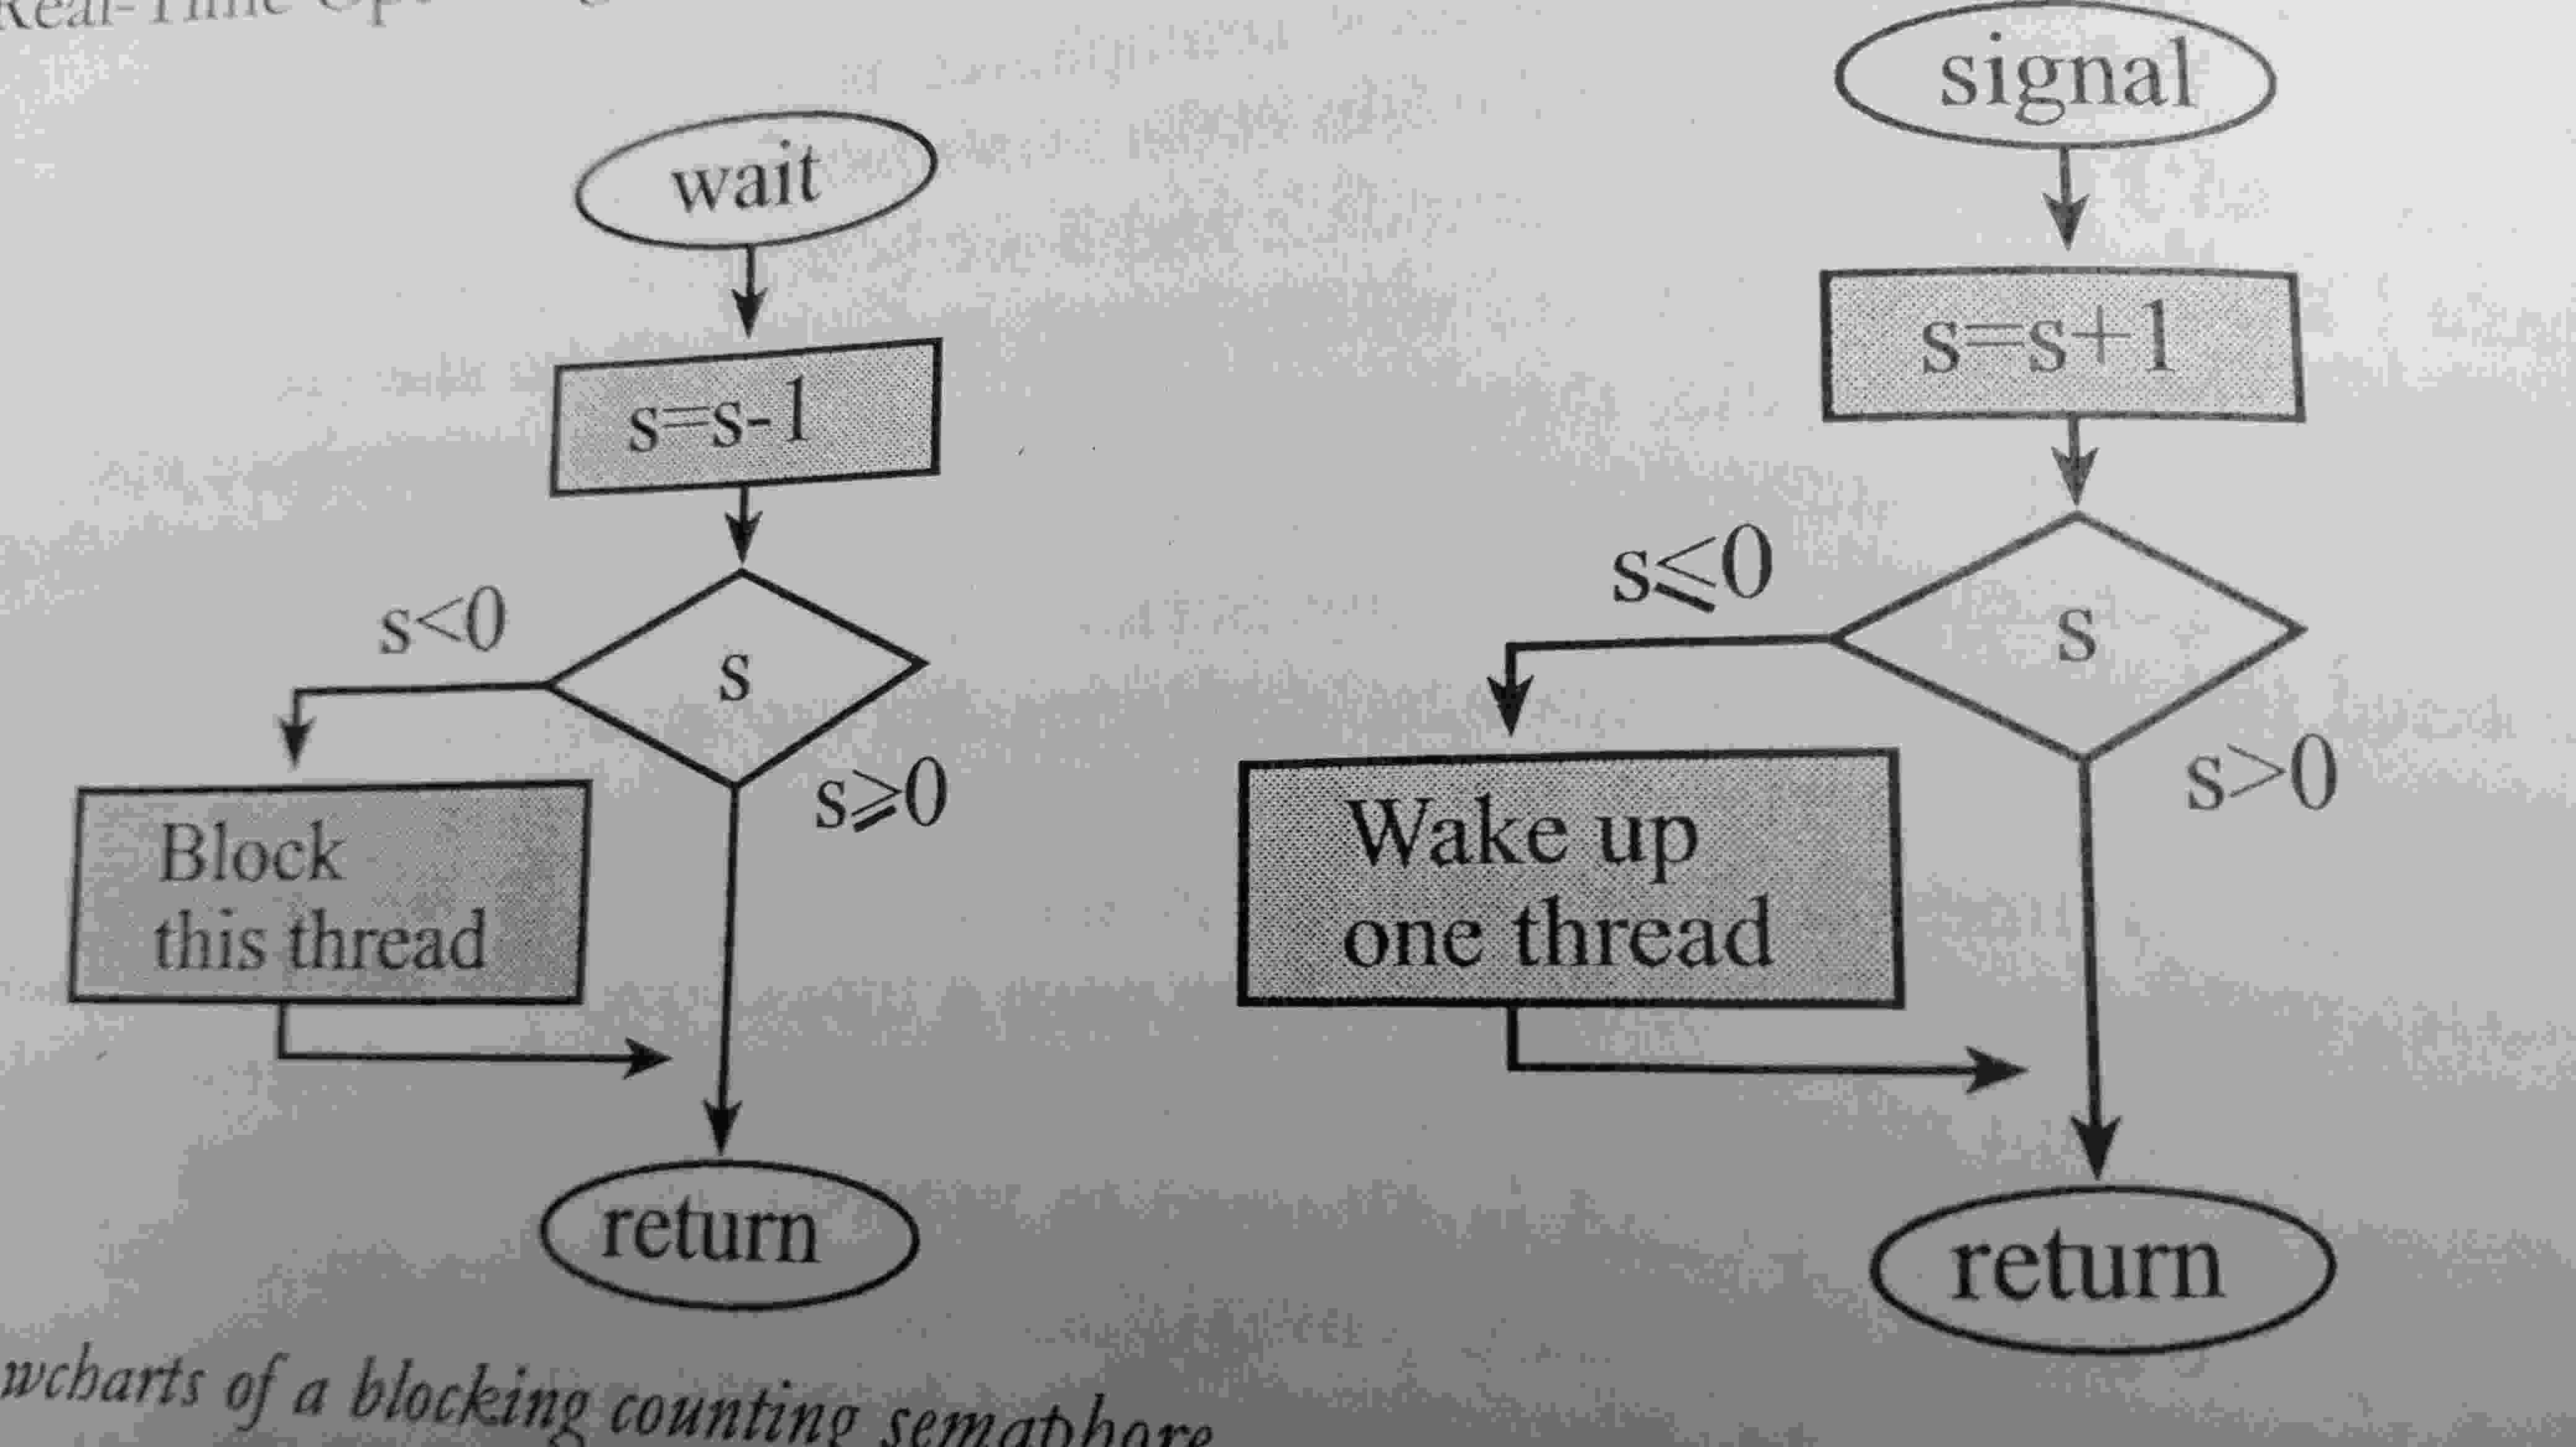
\includegraphics[scale=0.075]{img/OS_Wait_y_OS_Signal.jpg}
\caption{Diagramas de flujo para sem\'aforos bloqueantes}
\label{ValvanoVol3Pag176}
\end{center}
\end{figure}
La operaci\'on ``Block this thead'' establecer\'a el campo {\tt status} para que 
apunte al sem\'aforo, y despu\'es se suspende el thread como se muestra a continuaci\'on:
\begin{verbatim}
void OS_Wait(long *s){
  OS_DisableInterrupts();
  *s=*s-1;
  if(*s<0){// the ''Block this thread'' operation
    RunPt->status=s;          // reason it is blocked
    OS_Suspend();
  }
  OS_EnableInterrupts();
}
\end{verbatim}
La operaci\'on ``wakeup one thread'' ser\'a buscar de entre todos los TCBs uno 
que tenga un {\tt status} igual al sem\'aforo y despertarlo:
\begin{verbatim}
void OS_Signal(long *s){
  long st;
  tcbType *pt;
  st=StartCritical();
  *s=*s+1;
  if(*s<=0){// the ''wakeup one thread'' operation
    pt=RunPt->next;
    while(pt->status!=s) pt=pt->next;
    pt->status=0;             // wakeup this one
  }
  EndCritical(st);
}
\end{verbatim}
Las dos funciones anteriores se usan durante la opreaci\'on de los 
sem\'aforos. Para inicializar los sem\'aforos se usa la funci\'on
\begin{verbatim}
void OS_Semaphore_Init(long *s, long value){
  *s=value;
}
\end{verbatim}

Por otra parte, la funci\'on {\tt OS}$\_${\tt Suspend()} fue tomada 
del libro \cite{Valvano}, p\'ag. 174.
\begin{verbatim}
void OS_Suspend(void){
  NVIC_ST_CURRENT_R=0;         // clear counter
  NVIC_INT_CTRL_R=0x04000000;  // trigger SysTick interrupt
}
\end{verbatim}
y las funciones {\tt StartCritical()} y {\tt EndCritical(long)} est\'an 
escritas en lenguaje ensamblador en el archivo {\tt osasm.s}
\begin{verbatim}
;*********** StartCritical************************
; make a copy of previous I bit, disable interrupts
; inputs:  none
; outputs: previous I bit
StartCritical
        MRS     R0, PRIMASK        ; Set prio int mask to mask all (except faults)
        CPSID   I
        BX      LR


;*********** EndCritical************************
; using the copy of previous I bit, restore I bit to previous value
; inputs:  previous I bit
; outputs: none
EndCritical
        MSR     PRIMASK, R0
        BX      LR
\end{verbatim}
Lo anterior constituye una implementaci\'on de sem\'aforos bloqueantes para un  
sistema operativo construido a partir del archivo {\tt RTOS$\_$811.zip}, tomado del 
sitio web 
\begin{verbatim}
http://users.ece.utexas.edu/~valvano/arm
\end{verbatim}
que acompa\~na al libro \cite{Valvano}.

\eject
\begin{thebibliography}{9}
\bibitem{Brey}Barry B. Brey, ``Los Microprocesadores Intel, 
Arquitectura, programaci\'on e interfaces.'' Prentice-Hall 
3$^{a}$ Edici\'on, 1995.
\bibitem{Burns}Alan Burns, Andy Wellings, ``Real-Time Systems and 
Programming Languages'', Addison-Wesley, 3$^{\mbox{a}}$ Edici\'on, 
Pearson Education Limited 2001.
\bibitem{LDD3}Jonathan Corbet, Alessandro Rubini, Greg Kroah-Hartman, 
``Drivers en Linux, T\'ecnicas y soluciones para el desarrollo de 
Controladores'', O$^{\prime}$Reilly Anaya Multimedia, 2005.
\bibitem{Tanenbaum}Andrew S. Tanenbaum, ``Sistemas Operativos, 
Dise\~no e Implementaci\'on,'' Editorial Pearson, 2002.
\bibitem{Valvano}Jonathan W. Valvano, ``EMBEDDED SYSTEMS Volume 3, Real-Time Operating 
Systems for the ARM CORTEX-M3,'' 2012 Jonathan W. Valvano. ISBN-13:978-1466468863, 
ISBN-10:1466468866. 
\end{thebibliography}
\end{document}
